% ============================================================================
% 2026 CIE 全国 RISC-V 高水平创新及应用大赛（应用方向）
% 面向边缘 AI 大语言模型推理的 RISC-V 自定义 vdot 指令设计
% —— 基于“香山”昆明湖 V2 处理器架构
% 编译方式：xelatex
% ============================================================================
\documentclass[aspectratio=169]{beamer}

\usepackage{fontspec}
\defaultfontfeatures{Renderer=HarfBuzz}
\setmainfont{Heiti SC}
\setsansfont{Heiti SC}
\setmonofont{Andale Mono}[Scale=MatchLowercase]
\usepackage{xeCJK}
\setCJKmainfont{Heiti SC}
\setCJKsansfont{Heiti SC}
\setCJKmonofont{Heiti SC}

\usepackage{graphicx}
\usepackage{tikz}
\usetikzlibrary{arrows.meta,decorations.pathreplacing,fit,positioning,calc,shapes.geometric,shapes.misc,backgrounds,chains}
\usepackage{booktabs}
\usepackage{array}
\usepackage{xcolor}
\usepackage{amsmath,amssymb}
\usepackage{hyperref}
\usepackage{colortbl}
\usepackage{listings}

\usetheme{Madrid}
\usecolortheme{default}

\definecolor{ChinaRed}{RGB}{193,39,45}
\definecolor{DeepRed}{RGB}{140,20,25}
\definecolor{TechBlue}{RGB}{22,84,140}
\definecolor{LightGray}{RGB}{245,245,245}
\definecolor{DarkGray}{RGB}{70,70,70}
\definecolor{GoldAccent}{RGB}{212,168,67}
\definecolor{GreenOK}{RGB}{46,139,87}

\setbeamercolor{palette primary}{bg=ChinaRed,fg=white}
\setbeamercolor{palette secondary}{bg=DeepRed,fg=white}
\setbeamercolor{palette tertiary}{bg=TechBlue,fg=white}
\setbeamercolor{structure}{fg=ChinaRed}
\setbeamercolor{title}{fg=white}
\setbeamercolor{frametitle}{bg=ChinaRed,fg=white}
\setbeamercolor{block title}{bg=TechBlue,fg=white}
\setbeamercolor{block body}{bg=LightGray,fg=black}
\setbeamercolor{block title alerted}{bg=DeepRed,fg=white}
\setbeamercolor{block body alerted}{bg=LightGray,fg=black}

\setbeamertemplate{navigation symbols}{}
\setbeamertemplate{itemize items}[circle]
\setbeamertemplate{blocks}[rounded][shadow=false]

\setbeamerfont{frametitle}{size=\Large,series=\bfseries}
\setbeamerfont{title}{size=\LARGE,series=\bfseries}

% 压缩列表垂直间距，避免内容溢出底部
\AtBeginEnvironment{itemize}{\setlength{\itemsep}{1pt}}
\AtBeginEnvironment{enumerate}{\setlength{\itemsep}{1pt}}

\setbeamertemplate{footline}{%
  \leavevmode%
  \hbox{%
  \begin{beamercolorbox}[wd=.98\paperwidth,ht=2.6ex,dp=1.2ex,right]{footline}%
    \usebeamerfont{footline}\textcolor{DarkGray}{\scriptsize 2026 CIE RISC-V 大赛 · 应用方向 \hspace{2em}\insertframenumber\,/\,\inserttotalframenumber}\hspace{1em}%
  \end{beamercolorbox}}%
}

% 小表格工具（不用 float 环境，兼容 fragile 帧）
\newcommand{\smalltable}[1]{\par\centering\scriptsize #1\par}

\title[CIE2026 · vdot 设计]{\textbf{面向边缘 AI 大语言模型推理的 RISC-V 自定义 vdot 指令设计}}
\subtitle{—— 基于“香山”昆明湖 V2 处理器架构}
\author{参赛团队}
\date{2026 CIE 全国 RISC-V 高水平创新及应用大赛（应用方向）}

\begin{document}

% ===================== 封面 =====================
\begin{frame}[plain]
\begin{tikzpicture}[remember picture,overlay]
  \fill[ChinaRed] (current page.south west) rectangle (current page.north east);
  \fill[DeepRed,opacity=0.35] ([yshift=-1.5cm]current page.north west) rectangle (current page.north east);
  \foreach \i in {1,...,7}{
    \draw[white,opacity=0.08,line width=1.2pt]
      ([xshift=1.5cm*\i, yshift=-1cm]current page.south west) --
      ([xshift=1.5cm*\i+3cm, yshift=1cm]current page.south west);
  }
\end{tikzpicture}
\begin{center}
  \vspace{1.2cm}
  {\color{white}\Huge\bfseries 面向边缘 AI 大语言模型推理的}\\[0.25cm]
  {\color{white}\Huge\bfseries RISC-V 自定义 vdot 指令设计}\\[0.6cm]
  {\color{white!92!black}\large —— 基于“香山”昆明湖 V2 处理器架构}\\[1.6cm]
  {\color{white}\normalsize 2026 CIE 全国 RISC-V 高水平创新及应用大赛（应用方向）}\\[0.4cm]
  {\color{white!80!black}\small \today}
\end{center}
\end{frame}

% ===================== 目录 =====================
\begin{frame}{目录}
\tableofcontents
\end{frame}

% ============================================================
\section{需求分析与方案总览}
% ============================================================

% ---- 背景 ----
\begin{frame}{背景：点积是 LLM 推理的性能与能效瓶颈}
\begin{columns}[T]
\begin{column}{0.56\textwidth}
\textbf{点积（Dot Product）是深度学习最核心的计算内核}
\begin{itemize}
  \item \textbf{Transformer LLM}：自注意力 QK\textsuperscript{T} 与 AV 矩阵乘、FFN 两次 GEMM 均由海量点积构成；
  \item 以 GPT-2 为例，点积占\textbf{总计算量 70\% 以上}；
  \item 推荐系统中，78\% 的个性化推荐以点积作为核心排序指标；
  \item 边缘端部署时，点积执行效率直接决定\textbf{推理延迟、吞吐与能效}。
\end{itemize}
\end{column}
\begin{column}{0.42\textwidth}
\begin{block}{为什么是 INT8 量化（W8A8）}
\begin{itemize}
  \item \textbf{能效}：INT8 乘法器面积/功耗约为 FP32 的 $1/10\sim1/20$，算力密度（TOPS/mm\textsuperscript{2}）远高；
  \item \textbf{精度}：PTQ（per-tensor / per-channel / per-group）在 7B 以下模型可保持接近 FP16 精度；
  \item \textbf{生态}：llama.cpp / ggml、vLLM、TensorRT-LLM 均有成熟 INT8 量化与 GEMM kernel。
\end{itemize}
\end{block}
\textbf{结论：一条高效的 INT8 点积指令是边缘 LLM 推理的核心加速原语。}
\end{column}
\end{columns}
\end{frame}

% ---- 缺口 ----
\begin{frame}{缺口：RVV 1.0 没有原生整数点积指令}
\begin{columns}[T]
\begin{column}{0.5\textwidth}
\textbf{昆明湖 V2（Kunminghu V2）完整实现 RVV 1.0}
\begin{itemize}
  \item VLEN=128，SEW=8/16/32/64，支持掩码、尾元素、分段访存；
  \item 但 \textbf{RVV 1.0 没有一条“一组 INT8 元素点积累加”的原生指令}。
\end{itemize}
\textbf{现有做法的代价}
\begin{itemize}
  \item 组合 `vzext`/`vsext` + `vwmaccu` + 位宽加宽 + `vnsrl` 打包完成 INT8→INT32 累加，需\textbf{多条指令}；
  \item 指令数多、寄存器压力大、动态功耗高、吞吐低——K 维累加被“拆包+加宽+打包”胶水指令拖累。
\end{itemize}
\end{column}
\begin{column}{0.48\textwidth}
\begin{block}{行业对照：生态正走向“原生 vdot”}
\smalltable{%
\begin{tabular}{@{}p{3.0cm}p{3.1cm}@{}}
\toprule
来源 & 形态 \\
\midrule
RISC-V 官方 fast-track：\textbf{Zvdot4a8i / Zvqdotq} & 4×INT8 → INT32 累加，LLVM 已有支持 PR \\
SiFive：Xsfvdot / Xsfvqmacc & 自定义 INT8 矩阵乘-点积，QEMU/LLVM 已实现 \\
SpacemiT：XSMTVDot & 自定义向量点积，已合入 LLVM \\
香山昆明湖 & \textbf{无 —— 本赛题切入点} \\
\bottomrule
\end{tabular}}
\end{block}
\textbf{结论：为昆明湖 V2 设计并实现一条自定义 vdot 指令，既解决边缘 LLM 推理实际痛点，又与官方 Zvdot4a8i 方向一致，具备前瞻性与兼容路径。}
\end{column}
\end{columns}
\end{frame}

% ---- 目标 ----
\begin{frame}{目标与验收指标}
\begin{columns}[T]
\begin{column}{0.5\textwidth}
\begin{block}{四大目标}
\begin{enumerate}
  \item \textbf{设计指令}：4×INT8×INT8 → INT32 累加，遵循 RVV 1.0 语义，编码尽量对齐官方 Zvdot4a8i；
  \item \textbf{硬件集成}：解码接入 + 专用执行单元，极小面积换取数倍点积吞吐；
  \item \textbf{软件栈}：NEMU/Spike golden、LLVM/binutils、INT8 量化与 GEMM/注意力 kernel、端侧小模型推理演示；
  \item \textbf{验证评估}：指令级测试 + difftest + 基准（指令数/周期/吞吐/能效），给出可量化收益。
\end{enumerate}
\end{block}
\end{column}
\begin{column}{0.48\textwidth}
\begin{block}{指标（验收口径，相对 RVV vwmacc 基线）}
\smalltable{%
\begin{tabular}{@{}ll@{}}
\toprule
指标 & 目标值 \\
\midrule
指令数（INT8 GEMM 每输出元素） & 下降 $\ge 50\%$ \\
vdot 单元吞吐 & 1 条/周期（$\ge$4 组 INT32 累加/周期） \\
新增面积（含解码/调度） & $\le$ 全核 0.5\% \\
能效（INT8 GEMM TOPS/W） & 提升 $\ge 2\times$ \\
difftest 回归 & 全量通过，0 失配 \\
端侧小模型（$\le$2B）INT8 推理 & 可运行，per-token 延迟可复现 \\
\bottomrule
\end{tabular}}
\end{block}
\textbf{目标工作负载}：LLM 自注意力 QK\textsuperscript{T}/AV、FFN 两层 GEMM（K=4096）、Embedding/输出层、推荐双塔打分——vdot 每 4 元素一次点积，一条指令完成 4 组累加。
\end{column}
\end{columns}
\end{frame}

% ---- 技术路线 ----
\begin{frame}{总体技术路线（三阶段）}
\begin{center}
\begin{tikzpicture}[
  stage/.style={rectangle,rounded corners=3pt,draw=ChinaRed,fill=ChinaRed!8,minimum width=4.6cm,minimum height=0.8cm,align=center,font=\scriptsize},
  arrow/.style={-{Latex[length=2mm]},line width=1pt,ChinaRed}
]
  \node[stage] (s1) at (0,0) {\textbf{阶段一：环境部署与验证（基线）}\\ xs-env + kunminghu-v2 + NEMU + emu/difftest\\ riscv-tests / coremark 基线数据};
  \node[stage] (s2) at (0,-1.5) {\textbf{阶段二：vdot 设计与实现}\\ ISA 规格 → NEMU/Spike golden → RTL\\（解码+执行单元）→ 工具链 → 单元测试};
  \node[stage] (s3) at (0,-3.0) {\textbf{阶段三：协同仿真与评估}\\ difftest 回归 → 基准（micro/GEMM/端到端）\\ → 面积功耗时序评估 → 文档与提交};
  \draw[arrow] (0,-0.45) -- (0,-1.0);
  \draw[arrow] (0,-1.95) -- (0,-2.5);
\end{tikzpicture}
\hspace{0.7cm}
\begin{minipage}{0.52\textwidth}
\textbf{关键决策点}
\begin{enumerate}\footnotesize
  \item \textbf{指令形态}：RVV 1.0 编码空间的 4×INT8→INT32 点积（对齐 Zvdot4a8i 语义），继承 vl/vstart/掩码/尾元素语义；
  \item \textbf{硬件实现}：独立小执行单元挂入向量 ExeBlock，复用 VPRF 读/写回端口；备选扩展 VectorMul 数据通路；
  \item \textbf{软件顺序}：golden model（NEMU）先行 → 内联汇编/intrinsic 先行验证算法 → LLVM 完整支持后置；
  \item \textbf{验证策略}：golden-model 差分随机测试为主，difftest 全量回归兜底。
\end{enumerate}
\end{minipage}
\end{center}
\end{frame}

% ---- 创新点 ----
\begin{frame}{四大创新点}
\begin{columns}[T]
\begin{column}{0.5\textwidth}
\begin{block}{① 指令级创新}
面向 INT8 量化 LLM 推理的 \textbf{4×INT8→INT32 原生点积指令}，语义完整对齐 RVV 1.0（vl/vstart/掩码/尾元素/异常），编码与官方 fast-track 提案 Zvdot4a8i 一致，\textbf{具备直接演进为官方扩展的路径}。
\end{block}
\begin{block}{② 微架构创新}
以“极小面积开销换取数倍点积吞吐”为目标，给出\textbf{乘加阵列 + 加法树 + 累加器}数据通路设计、时延/吞吐权衡与面积功耗估算方法。
\end{block}
\end{column}
\begin{column}{0.5\textwidth}
\begin{block}{③ 系统级创新}
打通\textbf{“ISA → 硬件 → golden model → 编译器 → 量化 → GEMM kernel → LLM 推理”}全链路，交付可复现的端到端演示与评估数据，而非仅有 RTL 代码。
\end{block}
\begin{block}{④ 工程创新}
利用香山敏捷开发基础设施（difftest、随机差分测试、emu 周期仿真）建立\textbf{“指令语义 → 硬件 → 参考模型”三方一致}的可验证闭环。
\end{block}
\end{column}
\end{columns}
\end{frame}

% ============================================================
\section{指令集设计（ISA）}
% ============================================================

% ---- 设计原则 ----
\begin{frame}{ISA 设计原则与扩展命名}
\begin{columns}[T]
\begin{column}{0.55\textwidth}
\begin{block}{设计原则}
\begin{enumerate}
  \item \textbf{RVV 1.0 语义一致}：完整继承 `vl`/`vstart`/掩码/尾元素/异常语义，不发明新执行模型——与 `vsetvl` 无缝协作、golden 语义唯一、编译器可安全处理；
  \item \textbf{与官方方向对齐}：语义与助记符\textbf{完全对齐 Zvdot4a8i}，作为自定义扩展 `Xkhmvdot` 先行实现，官方发布后仅改扩展名即可平滑迁移；
  \item \textbf{最小侵入}：编码落在 RVV OP-V 主操作码（`1010111`）未占用空间，不触碰已实现 RVV 1.0 编码；
  \item \textbf{可验证}：每条指令有可执行伪代码与参考实现，支撑差分随机测试。
\end{enumerate}
\end{block}
\end{column}
\begin{column}{0.43\textwidth}
\begin{block}{扩展命名与使能}
\smalltable{%
\begin{tabular}{@{}ll@{}}
\toprule
项目 & 值 \\
\midrule
扩展名 & \texttt{Xkhmvdot} \\
助记符 & \texttt{vdota4}/\texttt{vdota4u}/\\
 & \texttt{vdota4su}/\texttt{vdota4us} \\
使能 & v1.0 恒使能（无独立 CSR） \\
对应官方 & \texttt{Zvdot4a8i}（Ratification 中） \\
\bottomrule
\end{tabular}}
\end{block}
\vspace{0.3em}
\textbf{8 条指令} = 4 种符号性 × 2 种操作数形式（vv / vx）。
\end{column}
\end{columns}
\end{frame}

% ---- 指令形态 ----
\begin{frame}{指令形态总览（8 条）}
\smalltable{%
\begin{tabular}{@{}llllll@{}}
\toprule
指令 & 操作数 & vs2 元素 & vs1 元素 & vd 累加 & 语义 \\
\midrule
\texttt{vdota4.vv} & vv & int8×4 & int8×4 & int32 & 有符号×有符号 \\
\texttt{vdota4u.vv} & vv & uint8×4 & uint8×4 & uint32 & 无符号×无符号 \\
\texttt{vdota4su.vv} & vv & int8×4 & uint8×4 & int32 & 有符号×无符号 \\
\texttt{vdota4us.vv} & vv & uint8×4 & int8×4 & int32 & 无符号×有符号 \\
\texttt{vdota4.vx} & vx & int8×4 & rs1 低 32 位 & int32 & 标量广播（4×int8） \\
\texttt{vdota4u.vx} & vx & uint8×4 & rs1 低 32 位 & uint32 & 标量广播 \\
\texttt{vdota4su.vx} & vx & int8×4 & rs1 低 32 位 & int32 & 标量广播 \\
\texttt{vdota4us.vx} & vx & uint8×4 & rs1 低 32 位 & int32 & 标量广播 \\
\bottomrule
\end{tabular}}
\vspace{0.6em}
\begin{itemize}
  \item \textbf{数据视图（关键约定）}：所有向量操作数以 \textbf{SEW=32 元素视图}访问（`vsew` 必须为 32）；每个 32 位元素内部重新解释为 \textbf{4 个打包的 8 位子元素}（little-endian，子元素 j 位于位 [8j, 8j+7]）。
  \item 元素计数（vl/vstart）单位是 32 位元素，\textbf{无 vl\%4 对齐约束}。
  \item \texttt{.vx} 形式将 rs1 视为“打包的 4 个 8 位元素”，用于权重/常量广播场景（如 QK\textsuperscript{T} 一侧固定向量、推荐打分）。
\end{itemize}
\end{frame}

% ---- 语义 ----
\begin{frame}[fragile]{语义精确定义（伪代码）}
\begin{columns}[T]
\begin{column}{0.5\textwidth}
\begin{block}{`vdota4.vv vd, vs2, vs1` 伪代码（权威定义）}
\scriptsize
\begin{verbatim}
SEW = 32
VLMAX = LMUL * VLEN / SEW
for i in [vstart, vl):
    if vm == 0 and mask[i] == 0:
        continue            # 该元素不更新
    acc = SExt32(vd[i])     # 读 vd 旧值
    for j in 0..3:
        a = Sub8(vs2[i], j) # 位 [8j, 8j+7]
        b = Sub8(vs1[i], j)
        acc = acc + a * b   # 乘积 16 位有符号
                            # 累加 32 位模 2^32 回绕
    vd[i] = acc
# 尾元素按 vta 策略处理
# vstart≠0 → illegal instruction（与昆明湖
# 所有向量算术指令一致）
\end{verbatim}
\end{block}
\end{column}
\begin{column}{0.48\textwidth}
\begin{block}{符号性矩阵}
\smalltable{%
\begin{tabular}{@{}llll@{}}
\toprule
变体 & vs2 & vs1 & 累加器 \\
\midrule
\texttt{vdota4} & s8 & s8 & s32 回绕 \\
\texttt{vdota4u} & u8 & u8 & u32 回绕 \\
\texttt{vdota4su} & s8 & u8 & s32 回绕 \\
\texttt{vdota4us} & u8 & s8 & s32 回绕 \\
\bottomrule
\end{tabular}}
\end{block}
\begin{block}{溢出与饱和策略}
\begin{itemize}\footnotesize
  \item \textbf{指令内}：单次点积范围 $\subseteq [-65536,\;+64516]$，\textbf{16 位有符号可完整表示，不溢出}；
  \item \textbf{跨指令累加}：32 位\textbf{模 $2^{32}$ 回绕}（wrapping），与 RVV `vadd.vv` 一致，\textbf{不做饱和}——INT8 GEMM 的 K 维累加（K=4096 $\to \approx 2^{28}$）在 int32 内天然安全。
\end{itemize}
\end{block}
\end{column}
\end{columns}
\end{frame}

% ---- vstart/掩码/尾元素 ----
\begin{frame}{vstart / 掩码 / 尾元素 与 RVV 交互约束}
\begin{columns}[T]
\begin{column}{0.55\textwidth}
\begin{block}{三种机制}
\smalltable{%
\begin{tabular}{@{}p{2.2cm}p{8.2cm}@{}}
\toprule
机制 & 定义 \\
\midrule
\texttt{vstart} & v1.0 与昆明湖一致：\texttt{vstart$\neq$0} 的向量算术指令在解码侧判 illegal instruction（RVV 规范允许仅支持 vstart=0）；正常执行由 `vsetvl` 清零，\textbf{vdot 无需新增机制} \\
掩码 \texttt{vm} & vm=0 时读掩码寄存器（EEW=1），掩码位 i 对应 32 位结果元素 i；掩码为 0 的元素不读源、不计算、不写 vd \\
尾元素 \texttt{vta} & v1.0 按 undisturbed 处理（写回旧值）；vta=0 同 undisturbed，由执行单元内 `Mgu` 统一处理 \\
\bottomrule
\end{tabular}}
\end{block}
\end{column}
\begin{column}{0.43\textwidth}
\begin{block}{与 RVV 1.0 交互约束（违反即 illegal）}
\smalltable{%
\begin{tabular}{@{}cl@{}}
\toprule
\# & 约束 \\
\midrule
C1 & `vsew` 必须为 32 \\
C2 & VLMAX $\ge$ 1 且寄存器组不越界（LMUL $\in\{1,2,4,8\}$） \\
C3 & 向量扩展已使能（`mstatus.VS` $\neq$ Off） \\
C4 & 编码落入已定义空间但组合未定义 → illegal \\
\bottomrule
\end{tabular}}
\end{block}
\textbf{除上述外}：不产生任何访存、无副作用 CSR 更新、无特权级限制，任何模式下可执行（与 RVV 算术指令一致）。
\end{column}
\end{columns}
\end{frame}

% ---- 编码 ----
\begin{frame}{编码（RVV OP-V 空间）}
\begin{columns}[T]
\begin{column}{0.52\textwidth}
\textbf{编码模板}：OP-V 主操作码 `1010111`（0x57）
\begin{center}
\scriptsize
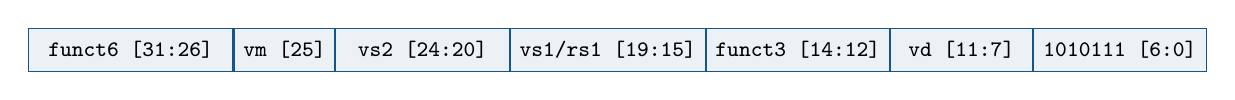
\begin{tikzpicture}[
  bit/.style={draw=TechBlue,fill=TechBlue!8,minimum height=0.55cm,font=\footnotesize\ttfamily}
]
  \node[bit,minimum width=2.6cm] (f6) at (0,0) {funct6 [31:26]};
  \node[bit,minimum width=0.9cm,right=0pt of f6] (vm) {vm [25]};
  \node[bit,minimum width=2.2cm,right=0pt of vm] (vs2) {vs2 [24:20]};
  \node[bit,minimum width=2.2cm,right=0pt of vs2] (vs1) {vs1/rs1 [19:15]};
  \node[bit,minimum width=1.4cm,right=0pt of vs1] (f3) {funct3 [14:12]};
  \node[bit,minimum width=1.8cm,right=0pt of f3] (vd) {vd [11:7]};
  \node[bit,minimum width=2.2cm,right=0pt of vd] (op) {1010111 [6:0]};
\end{tikzpicture}
\end{center}
\begin{itemize}
  \item \textbf{funct3 选型}：乘累加/宽乘累加族（`vmacc`/`vwmacc`/`vwmaccu`）统一使用 \texttt{010}（vv）/ \texttt{110}（vx）；vdot 语义上属“打包 4 元素宽乘累加”，故采用同类别，与官方 Zvdot4a8i 方向一致；
  \item \texttt{vm}=0 掩码使能；vv 形式 vs1 为向量，vx 形式为 rs1。
\end{itemize}
\end{column}
\begin{column}{0.46\textwidth}
\begin{block}{v1.0 编码定稿（已与实现同步）}
\smalltable{%
\begin{tabular}{@{}llll@{}}
\toprule
指令 & funct6 & funct3 & 状态 \\
\midrule
\texttt{vdota4.vv} & \texttt{111001} & 010 & \cellcolor{GreenOK!25}\textbf{$\checkmark$ 已实现} \\
\texttt{vdota4.vx} & \texttt{111001} & 110 & $\square$ 预留 \\
\texttt{vdota4u.vv} & \texttt{010100} & 010 & $\square$ 预留 \\
\texttt{vdota4u.vx} & \texttt{010100} & 110 & $\square$ 预留 \\
\texttt{vdota4su.vv} & \texttt{010101} & 010 & $\square$ 预留 \\
\texttt{vdota4su.vx} & \texttt{010101} & 110 & $\square$ 预留 \\
\texttt{vdota4us.vv} & \texttt{010110} & 010 & $\square$ 预留 \\
\texttt{vdota4us.vx} & \texttt{010110} & 110 & $\square$ 预留 \\
\bottomrule
\end{tabular}}
\end{block}
\textbf{编码核对已完成}：\texttt{111001} 经脚本扫描 rocket-chip 全部 OP-V BitPat + 香山自建表，\textbf{无冲突}（与 \texttt{VWMACCU\_VV} 同格式）；剩余核对项（官方定稿比对、反汇编 round-trip）待官方 Zvdot4a8i 发布/工具链落地时执行。
\end{column}
\end{columns}
\end{frame}

% ---- 行为汇总 ----
\begin{frame}{指令行为汇总（验证测试矩阵依据）}
\smalltable{%
\begin{tabular}{@{}ll@{}}
\toprule
场景 & 期望行为 \\
\midrule
正常 vv，vl=VLMAX & 全量计算，结果正确 \\
vl=0 & 无操作，vd 不变 \\
掩码全 0 / 部分 1 & vd 不变 / 仅掩码位=1 元素更新 \\
\texttt{vstart} $>$ 0 & \textbf{illegal instruction}（与昆明湖所有向量算术指令一致） \\
尾元素（i $\in [vl,\text{VLMAX})$） & 按 vta 策略（undisturbed/agnostic） \\
符号混合变体（su/us） & 按符号矩阵计算 \\
溢出回绕 & 模 $2^{32}$ 回绕（可构造边界用例） \\
SEW$\neq$32（8/16/64）、VS=Off、未定义编码 & illegal instruction \\
vx 形式 & rs1 低位 32 位作为打包 4×8bit 广播 \\
\bottomrule
\end{tabular}}
\vspace{0.6em}
\textbf{演进路径}：v1.0（本赛题交付，8 条指令恒使能）→ v1.1（扩展使能 CSR，虚拟化/多核选择性使能）→ v2.0（官方 Zvdot4a8i 发布后切换官方编码与扩展名；增加饱和变体、INT8×INT8→INT64 长累加对齐 Zvqdotq）。
\end{frame}

% ============================================================
\section{微架构设计}
% ============================================================

% ---- 总体思路 ----
\begin{frame}{微架构设计目标与总体思路}
\begin{columns}[T]
\begin{column}{0.52\textwidth}
\smalltable{%
\begin{tabular}{@{}lll@{}}
\toprule
目标 & 约束 & 策略 \\
\midrule
极小面积开销 & $\le$ 全核 0.5\% & 8×8 乘法阵列 + 加法树 + 32 位累加器 \\
数倍吞吐 & 1 条/周期 & 乘加阵列流水化，独立 FU \\
最小侵入 & 不动前端/访存/ROB & 仅改解码表+FuType+新单元+写回端口 \\
RVV 语义完整 & vl/vstart/掩码/尾/异常 & 复用向量后端既有机制 \\
\bottomrule
\end{tabular}}
\vspace{0.4em}
\begin{itemize}
  \item 源码基线：\texttt{kunminghu-v2} 分支 commit \texttt{e12436c7}（2026-08-14）；
  \item 结构提示：向量执行单元实际在 \texttt{backend/fu/wrapper/}（VIAluFix/VIMacU/VIDiv/VIPU/VPPU/...），公共框架在 \texttt{backend/fu/vector/}（VecPipedFuncUnit/Mgu/...）；
  \item 昆明湖\textbf{没有任何现成自定义指令钩子}（无 xvld/xvst/XCustom），vdot 必须走完整标准链路。
\end{itemize}
\end{column}
\begin{column}{0.46\textwidth}
\begin{block}{总体位置（示意）}
\centering
\begin{tikzpicture}[
  box/.style={rectangle,draw=TechBlue,rounded corners=2pt,minimum height=0.5cm,font=\scriptsize,align=center},
  new/.style={rectangle,draw=ChinaRed,rounded corners=2pt,minimum height=0.5cm,font=\scriptsize,align=center,fill=ChinaRed!12,thick}
]
  \node[box,minimum width=6.2cm] (fe) {前端 → 译码/重命名/分发};
  \node[box,minimum width=6.2cm,below=0.25cm of fe] (blk) {整数/浮点/访存 ExeBlock \ldots};
  \node[box,minimum width=6.2cm,below=0.25cm of blk] (vblk) {向量 ExeBlock（VfuCluster）};
  \node[box,minimum width=5.9cm,below=0.15cm of vblk,text width=5.7cm] (fus) {[VectorALU] [VectorShift] [VectorPermute] {\\} [VectorMul] [VectorDiv] \textcolor{ChinaRed}{\textbf{[vdot 单元★]}}};
  \node[box,minimum width=6.2cm,below=0.25cm of fus] (rob) {ROB 提交 → difftest → 写回状态};
  \draw[-{Latex[length=1.5mm]},line width=0.6pt] (fe)--(blk);
  \draw[-{Latex[length=1.5mm]},line width=0.6pt] (blk)--(vblk);
  \draw[-{Latex[length=1.5mm]},line width=0.6pt] (vblk)--(fus);
  \draw[-{Latex[length=1.5mm]},line width=0.6pt] (fus)--(rob);
  \node[below=0.15cm of rob,font=\scriptsize,text=ChinaRed] {共享 VPRF 读/写端口、writeback 端口};
\end{tikzpicture}
\end{block}
\end{column}
\end{columns}
\end{frame}

% ---- 解码接入 ----
\begin{frame}{解码接入（遵循昆明湖既有 RVV 链路）}
以 `vwmaccu.vv` 为样板，每环均已定位：
\begin{enumerate}\footnotesize
  \item \textbf{编码 BitPat}：\texttt{Instructions.scala} 登记 \texttt{VDOT\_VV = BitPat("b111001???????????010?????1010111")}（v1.0 已实现）；
  \item \textbf{解码表}：\texttt{VecDecoder.scala} 加入 \texttt{VDOTA4\_VV -> OPMVV(T, FuType.vdot, VdotType.vdota4, F, T, F, UopSplitType.VEC\_VVV)}——每 128-bit 输出 4×32bit 结果，\textbf{不真正加宽}，复用 \texttt{VEC\_VVV}（1 uop/lmul）；
  \item \textbf{fuOpType}：新增 \texttt{VdotType}（9-bit OpType：vs2/vs1/vd 符号 + format + 子操作码）；
  \item \textbf{FuType}：新增 \texttt{vdot}，同步加入 \texttt{vecOPI}/\texttt{vecArith}/\texttt{vecAll} 集合——\textbf{漏改任一集合会导致 dispatch 找不到可接受 EXU}；
  \item \textbf{illegal 检查}：\texttt{VecExceptionGen.scala} 补充 vdot 的 EEW/EMUL/重叠检查（数据视图特殊，不直接落入 `vdWideningInst`）；vstart$\neq$0 illegal 与执行侧兜底\textbf{自动覆盖}；
  \item \textbf{调度/写回}：\texttt{VdotCfg} 挂入 \textbf{VFEX0}（复用 3×VfRD + V0RD + VlRD 与 VfWB(0,0)）——\textbf{不新增 VPRF 端口号}。
\end{enumerate}
\begin{alertblock}{改动预估}
\footnotesize 硬件侧约 \textbf{600–1200 行 Scala}（Instructions +8 BitPat；VecDecoder +8 映射；VdotType +~30 行；FuType/FuConfig +~30 行；VdotU.scala 新文件 ~300–600 行；Vdot64b ~200–400 行；VecExceptionGen +10–40 行）。
\end{alertblock}
\end{frame}

% ---- 执行单元数据通路 ----
\begin{frame}{执行单元数据通路（VLEN=128，LMUL=1）}
\begin{center}
\begin{tikzpicture}[
  box/.style={rectangle,draw=TechBlue,rounded corners=2pt,minimum height=0.55cm,font=\scriptsize,align=center},
  mul/.style={rectangle,draw=ChinaRed,rounded corners=2pt,minimum height=0.5cm,font=\scriptsize,align=center,fill=ChinaRed!10},
  arr/.style={-{Latex[length=1.5mm]},line width=0.7pt}
]
  \node[box,minimum width=2.6cm] (v2) at (0,0) {\texttt{vs2[127:0]}\\16 × int8};
  \node[box,minimum width=2.6cm] (v1) at (0,-1.1) {\texttt{vs1[127:0]}\\16 × int8};
  \node[mul,minimum width=2.8cm] (mul16) at (4.6,-0.55) {16 个 8×8 乘法器};
  \node[box,minimum width=2.8cm] (tree) at (8.0,-0.55) {4 个 4:2 压缩/加法树};
  \node[box,minimum width=2.8cm] (acc) at (11.4,-0.55) {4 × int32 累加（回绕）};
  \node[box,minimum width=2.8cm] (wb) at (14.2,0.5) {写回 vd（掩码/尾处理后）};
  \node[box,minimum width=2.8cm] (old) at (11.4,0.9) {vd 旧值（4 × int32）};
  \draw[arr] (v2) -- node[above,font=\scriptsize]{128 bit} (mul16);
  \draw[arr] (v1) -- (mul16);
  \draw[arr] (mul16) -- node[above,font=\scriptsize]{16-bit 乘积} (tree);
  \draw[arr] (tree) -- node[above,font=\scriptsize]{4 × int32 部分和} (acc);
  \draw[arr] (old) -- (acc);
  \draw[arr] (acc) -- (wb);
  \node[below=0.55cm of mul16,font=\scriptsize\color{DarkGray}] {符号性由指令变体控制（输入 2 选 1 符号扩展）};
  \node[below=0.55cm of tree,font=\scriptsize\color{DarkGray}] {两组 4 乘积 → 两级加法，17 位无溢出和 $[-65536,64516]$};
\end{tikzpicture}
\end{center}
\begin{itemize}
  \item \textbf{多周期流水}：建议 \textbf{latency = 2}（与 VIMacCfg/CertainLatency(2)、yunsuan VIMac64b 两级寄存器结构同构；吞吐 1 条/周期，无结构冲突）；
  \item \textbf{掩码/尾/vstart}：由执行单元内 \texttt{Mgu}（mask/tail merge unit）统一处理——vdot 直接复用，无新逻辑；
  \item \textbf{LMUL}：1/2/4/8 均可寻址（int32 元素视图，无加宽比限制）；LMUL>1 按寄存器组分段执行（每周期一个 128-bit 片段），吞吐相应降低。
\end{itemize}
\end{frame}

% ---- 性能建模 ----
\begin{frame}{性能建模与面积/功耗/时序估算}
\vspace{-0.65em}
\begin{columns}[T]
\begin{column}{0.48\textwidth}
\begin{block}{吞吐与数据率（设计预估）}
\smalltable{%
\begin{tabular}{@{}ll@{}}
\toprule
参数 & 值 \\
\midrule
VLEN / 数据通路宽度 & 128 bit \\
每周期点积组数 & 4（16 对 8×8 乘加） \\
吞吐 & 1 条/周期（16 MAC/周期） \\
时延 & 2 周期（建议） \\
uop 拆分 & \texttt{VEC\_VVV}（1 uop/lmul） \\
面积（估算） & 乘法器 ~3.2k + 加法树/累加 ~2k 门 \\
\bottomrule
\end{tabular}}
\end{block}
\begin{block}{相对 RVV 1.0 基线的收益（预估）}
\smalltable{%
\begin{tabular}{@{}llll@{}}
\toprule
指标 & RVV 组合 & vdota4 & 提升 \\
\midrule
指令数/4×4 & ~8–12 & 1 & $\ge 8\times$ \\
动态功耗 & 高 & 低 & 显著 \\
寄存器压力 & 高 & 低 & 减少 ~50\% \\
\bottomrule
\end{tabular}}
\end{block}
\end{column}
\begin{column}{0.5\textwidth}
\begin{block}{面积 / 功耗 / 时序估算方法}
\begin{itemize}\footnotesize
  \item \textbf{面积}：vdot 单元独立综合（Synopsys DC 或开源 OpenROAD），报告面积 ÷ 全核估计面积，目标 $\le 0.5\%$；
  \item \textbf{功耗}：综合后功耗报告（基准波形回标 switching activity）→ TOPS/W 对比；
  \item \textbf{时序}：8×8 乘法（~0.5–1ns@28nm）+ 加法树 + 32 位累加，目标频率按昆明湖主频（1–2GHz 假设，注明口径）；
  \item \textbf{口径}：所有数字注明工艺、库、温度/电压条件，保证可复现可审计。
\end{itemize}
\end{block}
\begin{block}{备选实现方案}
\smalltable{%
\begin{tabular}{@{}llll@{}}
\toprule
方案 & 描述 & 优点 & 缺点 \\
\midrule
\textbf{A（默认）} & 独立 \texttt{VdotU} + yunsuan \texttt{Vdot64b}，2 拍，挂 VFEX0 & 解耦、风险最小 & 需新增核心 \\
B & 扩展 \texttt{VIMac64b} 加积点模式 & 复用 Booth/Wallace，面积最小 & 侵入 VIMac 核心 \\
C & VIAluFix 多周期微码 & 无新单元 & 吞吐低 \\
\bottomrule
\end{tabular}}
\end{block}
\end{column}
\end{columns}
\end{frame}

% ---- 改动点清单 ----
\begin{frame}{改动点清单（代码级，kunminghu-v2 @ e12436c）}
\smalltable{%
\begin{tabular}{@{}cp{6.4cm}cl@{}}
\toprule
\# & 文件/模块（相对 \texttt{src/main/scala/}） & 改动 & 估计量 \\
\midrule
1 & \texttt{backend/decode/Instructions.scala} & 新增 \texttt{object Xkhmvdot}（8 条 BitPat） & +8 条目 \\
2 & \texttt{backend/decode/VecDecoder.scala} & 新增 8 条 OPMVV/OPMVX 映射（\texttt{VEC\_VVV}） & +8 映射 \\
3 & yunsuan \texttt{package.scala} + Opcode & 新增 \texttt{VdotType}（9-bit OpType） & +~30 行 \\
4 & \texttt{backend/fu/FuType.scala} & 新增 \texttt{vdot}，同步集合 & +~8 行 \\
5 & \texttt{backend/fu/FuConfig.scala} & 新增 \texttt{VdotCfg}（仿 VimacCfg）+ 谓词 & +~20 行 \\
6 & \texttt{Parameters.scala}（vfSchdParams:449） & \texttt{VdotCfg} 加入 VFEX0 & +1 行 \\
7 & \texttt{backend/fu/wrapper/VdotU.scala}（新建） & VecPipedFuncUnit + 2×64-bit 核心 + Mgu & ~300–600 行 \\
8 & yunsuan \texttt{vectorIMAC/Vdot64b.scala}（新建） & 8×8 乘法 + 加法树 + int32 累加 & ~200–400 行 \\
9 & \texttt{backend/decode/VecExceptionGen.scala} & vdot 的 EEW/EMUL/重叠检查 & +10–40 行 \\
10 & \texttt{DecodeUnitComp.scala} / UopInfoGen & 复用 \texttt{VEC\_VVV}，\textbf{无需改动} & 0 \\
11 & 测试 & Vdot64bSpec + decode 单测 + 回归 & 中 \\
12 & NEMU（外部仓库） & 8 条指令语义 + 编码注册 & 中 \\
13 & difftest & \textbf{无需改动}（DiffInstrCommit 已覆盖） & 0 \\
\bottomrule
\end{tabular}}
\vspace{0.4em}
\textbf{合计：硬件侧约 600–1200 行 Scala + NEMU 实现与测试}。VPRF 复用现有端口（6R/4W，自动推导），\textbf{面积零增长}。
\end{frame}

% ============================================================
\section{软件栈与工具链}
% ============================================================

% ---- 软件栈总览 ----
\begin{frame}{软件栈总览与推进顺序}
\vspace{-0.45em}
\begin{columns}[T]
\begin{column}{0.44\textwidth}
\begin{block}{软件栈（六层）}
\centering
\begin{tikzpicture}[
  l/.style={rectangle,rounded corners=2pt,minimum width=4.8cm,minimum height=0.52cm,font=\scriptsize,align=center}
]
  \node[l,fill=ChinaRed!85,text=white] (a) {应用层：LLM 推理（llama.cpp/自研）· 推荐打分 · 基准};
  \node[l,fill=TechBlue,text=white] at (0,-0.72) {Kernel 层：INT8 GEMM/GEMV · QK\textsuperscript{T}/AV · 量化/反量化};
  \node[l,fill=DarkGray,text=white] at (0,-1.42) {Intrinsic：\texttt{\_\_riscv\_vdota4\_*} / 内联汇编 / C fallback};
  \node[l,fill=GoldAccent!85!black,text=white] at (0,-2.12) {编译器：LLVM（Xkhmvdot subtarget + intrinsic + MC）· binutils};
  \node[l,fill=ChinaRed!60,text=white] at (0,-2.82) {模拟层：NEMU（difftest golden）· Spike · 软件仿真器};
  \node[l,fill=TechBlue!60,text=white] at (0,-3.52) {硬件层：昆明湖 V2 RTL（vdot 执行单元）};
  \draw[-{Latex[length=1.5mm]},line width=0.5pt,DarkGray!40] (0,-0.35)--(0,-0.58);
  \draw[-{Latex[length=1.5mm]},line width=0.5pt,DarkGray!40] (0,-1.05)--(0,-1.28);
  \draw[-{Latex[length=1.5mm]},line width=0.5pt,DarkGray!40] (0,-1.75)--(0,-1.98);
  \draw[-{Latex[length=1.5mm]},line width=0.5pt,DarkGray!40] (0,-2.45)--(0,-2.68);
  \draw[-{Latex[length=1.5mm]},line width=0.5pt,DarkGray!40] (0,-3.15)--(0,-3.38);
\end{tikzpicture}
\end{block}
\end{column}
\begin{column}{0.54\textwidth}
\begin{block}{推进顺序原则}
\textbf{模拟层（golden model）先行 → intrinsic/内联汇编让算法组先写 kernel → 编译器支持后置 → 最后集成 LLM 推理。}
\end{block}
\begin{block}{golden model}
\begin{itemize}
  \item \textbf{NEMU}：按 02 §4.2 伪代码实现 8 条指令语义；\textbf{必须在解码表/扩展注册处登记自定义编码}（否则报 illegal 与硬件失配）；差异点清单随代码交付；
  \item \textbf{Spike}：\texttt{riscv/insns/vdota4*.h} + 解码表 + 扩展名注册（\texttt{-march=rv64gcv\_xkhmvdot}）；
  \item \textbf{软件仿真器}（开发期 fallback）：逐元素仿真，作为“第 3 个参考实现”参与随机差分对拍。
\end{itemize}
\end{block}
\begin{block}{编译器}
\textbf{LLVM}：参考已合入上游的 Zvdot4a8i PR（\#184089）、XSMTVDot、Xsfvdot 模式——Feature + intrinsic 声明 + MC 编码 + 测试；\textbf{binutils} 可后置（LLVM MC + 内置汇编器已覆盖开发测试需求）。
\end{block}
\end{column}
\end{columns}
\end{frame}

% ---- 量化与 kernel ----
\begin{frame}[fragile]{量化方案与 INT8 GEMM kernel}
\begin{columns}[T]
\begin{column}{0.48\textwidth}
\begin{block}{量化策略分级}
\smalltable{%
\begin{tabular}{@{}llll@{}}
\toprule
级别 & 粒度 & 精度 & vdot 适配 \\
\midrule
L1 & per-tensor & 一般 & 直接支持 \\
L2 & per-channel & 好 & 权重打包带 scale 向量 \\
L3 & per-group & 最好 & 反量化循环按 group 取 scale \\
\bottomrule
\end{tabular}}
\end{block}
\begin{itemize}
  \item v1.0 交付 \textbf{L1 + L2}，L3 作扩展；对称 INT8 为默认；
  \item \textbf{反量化移出 K 循环}（K 维累加保持 int32，vdot 只承担最重乘加）；
  \item \textbf{权重打包}：每个 32 位字装 K 维方向相邻 4 个 int8（离线静态完成，运行时零开销）；K 非 4 倍数 padding 补 0。
\end{itemize}
\end{column}
\begin{column}{0.5\textwidth}
\begin{block}{INT8 GEMM/GEMV microkernel（核心交付）}
\scriptsize
\begin{verbatim}
// M=1 GEMV，K=4096，N 分块
for (n = 0; n < N; n += 4) {      // 4 个输出通道
  vint32m1_t acc = 0;
  for (k = 0; k < K; k += 4) {
    vint32m1_t xv = vle32(&x_packed[k/4]);   // 4×int8
    vint32m1_t wv = vle32(&W_packed[k/4][n/4]);
    acc = __riscv_vdota4_vv_i32m1(acc, xv, wv, VLMAX);
  }   // 一条指令 4 组点积
  // 反量化 + 写回
}
\end{verbatim}
\end{block}
\textbf{收益（理论）}：每 4×4 乘加由 ~8–12 条指令降为 1 条 vdota4 + 2 条 vle32，\textbf{指令数下降 $\ge$ 60\%，寄存器压力减半}。
\end{column}
\end{columns}
\end{frame}

% ---- LLM 集成 ----
\begin{frame}{注意力 kernel 与 LLM 推理集成}
\vspace{-0.55em}
\begin{columns}[T]
\begin{column}{0.5\textwidth}
\begin{block}{注意力 kernel}
\begin{itemize}
  \item \textbf{QK\textsuperscript{T}}：M=1（单 token），K=hdim（如 128/group），vdot 逐组点积 → fp32 → softmax；
  \item \textbf{AV}：S×V，vdot 累加 → 输出 token；
  \item 长序列分段（如 S=4096 按 chunk）控制寄存器与延迟。
\end{itemize}
\end{block}
\begin{block}{LLM 推理集成（两条路径）}
\smalltable{%
\begin{tabular}{@{}llll@{}}
\toprule
路径 & 说明 & 推荐度 \\
\midrule
\textbf{A. 自研轻量栈} & 注意力 + FFN + 量化 + $\le$2B 模型 INT8 & ★★★ 主交付 \\
B. llama.cpp/ggml & 替换 q8\_0 GEMM 向量化路径 & ★★ 加分项 \\
\bottomrule
\end{tabular}}
\end{block}
\textbf{建议}：路径 A 为主交付（可控、可演示、可复现）；路径 B 作为加分项贡献上游。
\end{column}
\begin{column}{0.48\textwidth}
\begin{block}{工具链打通顺序（依赖图）}
\centering
\begin{tikzpicture}[
  n/.style={rectangle,draw=TechBlue,rounded corners=2pt,minimum height=0.45cm,font=\scriptsize,align=center}
]
  \node[n] (s1) at (0,0) {1. 软件仿真器};
  \node[n] (s2) at (3.6,0) {2. NEMU 实现};
  \node[n] (s3) at (6.6,0) {3. difftest 对拍};
  \node[n] (s4) at (1.8,-0.9) {4. intrinsic + kernel};
  \node[n] (s5) at (4.6,-1.6) {5. LLVM 支持};
  \node[n] (s6) at (4.6,-2.5) {6. binutils（可后置）};
  \node[n,fill=ChinaRed!15] (s7) at (4.6,-3.4) {7. 基准 + LLM 演示};
  \draw[-{Latex[length=1.2mm]},line width=0.5pt] (s1)--(s2);
  \draw[-{Latex[length=1.2mm]},line width=0.5pt] (s2)--(s3);
  \draw[-{Latex[length=1.2mm]},line width=0.5pt] (s4)--(s2);
  \draw[-{Latex[length=1.2mm]},line width=0.5pt] (s4)--(s5);
  \draw[-{Latex[length=1.2mm]},line width=0.5pt] (s5)--(s6);
  \draw[-{Latex[length=1.2mm]},line width=0.5pt] (s6)--(s7);
  \draw[-{Latex[length=1.2mm]},line width=0.5pt] (s2) to[out=60,in=120] (s3);
\end{tikzpicture}
\end{block}
\begin{block}{软件侧交付物}
NEMU/Spike patch、软件仿真器、intrinsic 头文件、LLVM patch（目标合入上游）、打包器、GEMM/注意力 kernel、LLM 推理演示。
\end{block}
\end{column}
\end{columns}
\end{frame}

% ============================================================
\section{验证与评估方案}
% ============================================================

% ---- 验证层次 ----
\begin{frame}{验证目标与层次}
\begin{columns}[T]
\begin{column}{0.5\textwidth}
\smalltable{%
\begin{tabular}{@{}llll@{}}
\toprule
层次 & 对象 & 方法 & 通过标准 \\
\midrule
L0 指令语义 & 仿真器/NEMU/Spike & 指令级测试+随机差分 & 三方一致，100\% 通过 \\
L1 硬件功能 & vdot RTL & 定向+随机+difftest & difftest 0 失配 \\
L2 系统集成 & 昆明湖 V2 全核 & riscv-tests+向量测试+回归 & 无回归 \\
L3 性能/能效 & 单元/GEMM/LLM & 基准（口径见 §5） & 达到验收指标 \\
\bottomrule
\end{tabular}}
\vspace{0.4em}
\textbf{核心思想}：功能验证以\textbf{“三方一致 + difftest 兜底”}为核心；评估以\textbf{“可复现、口径明确”}为原则。
\end{column}
\begin{column}{0.48\textwidth}
\begin{block}{指令级测试矩阵（节选）}
\smalltable{%
\begin{tabular}{@{}ll@{}}
\toprule
类别 & 覆盖点 \\
\midrule
基本 & 4 符号性 × 2 形式 × 手工算例 \\
vl 边界 & vl=0、1..VLMAX-1、VLMAX、>VLMAX \\
掩码 & 全 1/0、交替、随机 \\
vstart & =0 正常；$\neq$0 → illegal \\
尾策略 & vta=0/1、尾元素旧值保持 \\
溢出 & 全 127、全 -128、多轮累加 \\
非法 & SEW$\in${8,16,64}、VS=Off、未定义编码 \\
寄存器组 & LMUL=1/2/4/8、越界检测 \\
数据布局 & 打包子元素边界、大小端 \\
vx 形式 & rs1 各 4 字节组合、符号性 \\
随机 & 随机 vl/vstart/掩码/数据/符号性 \\
\bottomrule
\end{tabular}}
\end{block}
\end{column}
\end{columns}
\end{frame}

% ---- 随机差分与 difftest ----
\begin{frame}{随机差分（三方一致）与 difftest 协同仿真}
\vspace{-0.65em}
\begin{columns}[T]
\begin{column}{0.5\textwidth}
\begin{block}{随机差分测试}
\centering
\begin{tikzpicture}[
  n/.style={rectangle,draw=TechBlue,rounded corners=2pt,minimum height=0.45cm,font=\scriptsize,align=center}
]
  \node[n,fill=ChinaRed!12] (gen) at (0,0.4) {随机激励生成器\\（数据/vl/vstart/掩码/符号性/LMUL）};
  \node[n] (r1) at (0,-1.0) {软件仿真器（参考 1）};
  \node[n] (r2) at (0,-1.7) {NEMU/Spike（参考 2）};
  \node[n] (r3) at (0,-2.4) {RTL 仿真（参考 3，emu/VCS）};
  \node[n,fill=GreenOK!15] (cmp) at (0,-3.3) {结果比对（vd 全寄存器 + 异常标志）\\失配即报错并最小化复现};
  \draw[-{Latex[length=1.2mm]},line width=0.5pt] (gen)--(r1);
  \draw[-{Latex[length=1.2mm]},line width=0.5pt] (gen)--(r2);
  \draw[-{Latex[length=1.2mm]},line width=0.5pt] (gen)--(r3);
  \draw[-{Latex[length=1.2mm]},line width=0.5pt] (r1)--(cmp);
  \draw[-{Latex[length=1.2mm]},line width=0.5pt] (r2)--(cmp);
  \draw[-{Latex[length=1.2mm]},line width=0.5pt] (r3)--(cmp);
\end{tikzpicture}
\end{block}
\begin{itemize}
  \item 覆盖：SEW×LMUL×vl×vstart×掩码×符号性×数据模式；
  \item 数量：随机用例 $\ge$ 1 万条，\texttt{--seed} 可复现；
  \item 失配用例自动 delta-debug 生成最小复现。
\end{itemize}
\end{column}
\begin{column}{0.48\textwidth}
\begin{block}{difftest 协同仿真}
\begin{itemize}
  \item 框架：\texttt{emu --diff riscv64-nemu-interpreter-so}；
  \item \textbf{前提}：NEMU 已实现 8 条指令，否则必然失配；
  \item \textbf{测试负载}：riscv-tests 全量 / 自研向量测试集 / 随机差分镜像 / kernel 冒烟（GEMM 与 fp32 参考比对误差界）/ LLM 推理冒烟（per-token 输出比对）；
  \item \textbf{通过标准}：全部 difftest 0 失配、0 死锁。
\end{itemize}
\end{block}
\begin{block}{回归策略与 CI}
\begin{itemize}
  \item 每日回归：L0 + L1 difftest 冒烟（固定 seed 集）；
  \item 提交前门禁：L0–L2 全量 + B1 基准（防性能回退，记录 commit → 指标曲线）。
\end{itemize}
\end{block}
\end{column}
\end{columns}
\end{frame}

% ---- 基准 ----
\begin{frame}{性能与能效基准（口径定义）}
\vspace{-0.65em}
\begin{columns}[T]
\begin{column}{0.5\textwidth}
\smalltable{%
\begin{tabular}{@{}llll@{}}
\toprule
基准 & 度量 & 对比对象 & 口径 \\
\midrule
B0 micro & 吞吐、时延 & vadd/vwmacc 基线 & RTL 计数/emu 周期 \\
B1 GEMM & 指令数、周期、寄存器压力 & vwmacc 组合 & emu 周期（同分块/打包） \\
B2 端到端 & per-token 延迟、吞吐 & FP16/INT8 基线 & emu 或实机 \\
B3 能效 & TOPS/W & vwmacc 组合路径 & 综合后功耗估算 \\
\bottomrule
\end{tabular}}
\vspace{0.4em}
\textbf{B1 指令数理论对比}（VLEN=128，LMUL=1，K=4）：
\smalltable{%
\begin{tabular}{@{}ll@{}}
\toprule
实现 & 每 4×4 乘加指令数 \\
\midrule
RVV 组合（vzext→vwmaccu→加宽→vnsrl） & ~8–12 条 \\
本设计 vdota4 & \textbf{1 条} \\
\bottomrule
\end{tabular}}
\end{column}
\begin{column}{0.48\textwidth}
\begin{block}{实验对照原则}
\begin{itemize}
  \item 同一 kernel 框架、量化参数、分块参数下，仅替换“点积原语”，保证对比公平；
  \item 数据可复现：固定 seed、固定镜像、记录环境（commit SHA、编译选项、仿真器版本）。
\end{itemize}
\end{block}
\begin{block}{面积/功耗/时序评估}
\begin{itemize}
  \item 面积：独立综合（DC 或 OpenROAD），占比 $\le$ 0.5\%；
  \item 功耗：波形回标 switching activity → TOPS/W；
  \item 时序：关键路径分析 vs 目标频率，不满足则流水切分（备选方案 B）。
\end{itemize}
\end{block}
\begin{block}{验收清单（对应指标）}
指令数下降 $\ge$50\%（B1 实测）· 吞吐 1 条/周期（B0）· 面积 $\le$0.5\%（综合报告）· 能效 $\ge$2×（B3）· difftest 0 失配（回归日志）· 端侧小模型可运行（B2 演示）。
\end{block}
\end{column}
\end{columns}
\end{frame}

% ============================================================
\section{实施计划与当前进度}
% ============================================================

% ---- 里程碑 ----
\begin{frame}{实施计划：里程碑总览（三阶段 + FPGA 加分项）}
\smalltable{%
\begin{tabular}{@{}llll@{}}
\toprule
阶段 & 目标 & 关键产出 & 退出标准 \\
\midrule
阶段一 环境部署与验证（2–3 人周） & 打通开发与仿真基线 & xs-env、emu、difftest 基线 & \texttt{emu} 跑通 riscv-tests/coremark，difftest 0 失配 \\
阶段二 vdot 设计与实现（5–7 人周） & 指令从规格到 RTL 落地 & ISA 定稿、golden、RTL、intrinsic、指令级测试 & 三方一致，difftest 冒烟通过 \\
阶段三 协同仿真与评估（3–4 人周） & 证明正确与收益 & 全量回归、B0–B3、面积报告、LLM 演示 & 验收清单全部达成 \\
阶段四 FPGA 原型验证（6–10 人周，加分） & 单卡运行 V4-Flash 同构模型 & vdot+香山子集核上板、INT8 GEMM 阵列 & 单卡 $\ge$50 token/s；多卡 EP 预估/实测 \\
\bottomrule
\end{tabular}}
\vspace{0.5em}
\begin{columns}[T]
\begin{column}{0.5\textwidth}
\textbf{关键路径}：1.2 → 1.4 → 2.3 → 2.5 → 3.1 → 3.2
\begin{itemize}
  \item \textbf{可并行支线}：golden/kernel（2.2/2.6/2.7）与 RTL（2.3–2.5）互不阻塞；LLVM（2.8）全程并行；
  \item 阶段二预留 1 周缓冲。
\end{itemize}
\end{column}
\begin{column}{0.48\textwidth}
\textbf{主要风险与缓解}
\begin{itemize}
  \item 官方编码冻结冲突 → 以官方为准切换（改动集中解码表+工具链）；
  \item 时序不满足 → 流水切分 / 扩展 VIMac64b 复用 2 级寄存器；
  \item difftest 失配 → 三方随机差分先行定位、失配自动最小化；
  \item LLVM 工作量超预期 → 内联汇编 intrinsic 保底；
  \item 源码/环境问题 → xs-env 官方流程 + 大赛答疑通道。
\end{itemize}
\end{column}
\end{columns}
\end{frame}

% ---- 交付物 ----
\begin{frame}[fragile]{最终交付物清单与提交}
\begin{columns}[T]
\begin{column}{0.52\textwidth}
\smalltable{%
\begin{tabular}{@{}ll@{}}
\toprule
类别 & 交付物 \\
\midrule
文档 & 设计文档套件（01–06）\\
RTL & 解码+执行单元+后端集成 patch（含单测）\\
Golden & NEMU/Spike patch + 软件仿真器\\
工具链 & LLVM patch + intrinsic 头文件 + 打包器\\
软件 & INT8 GEMM/注意力 kernel、量化脚本、LLM 演示\\
验证 & 指令级测试、随机差分、回归脚本与报告\\
评估 & B0–B3 报告（性能/能效/面积）\\
提交 & \texttt{my\_submission.txt}、PR 描述\\
\bottomrule
\end{tabular}}
\end{column}
\begin{column}{0.46\textwidth}
\begin{block}{\texttt{my\_submission.txt} 模板}
\footnotesize
\begin{verbatim}
team-name: （团队名称）
repo-url: github.com/...git
github-username: （用户名）
contact-email: （邮箱）
project-description: 面向边缘AI LLM
  推理的RISC-V自定义vdot指令（4×
  INT8→INT32点积）设计，基于香山
  昆明湖V2实现解码、执行单元与软件
  栈，difftest验证+GEMM/端到端
  基准评估
university: （学校/单位）
advisor: （指导老师）
team-members: 成员1(架构), 成员2
  (硬件), 成员3(软件), 成员4(验证)
notes: 语义对齐RISC-V官方Zvdot4a8i
  fast-track提案，平滑演进路径
\end{verbatim}
\end{block}
\end{column}
\end{columns}
\end{frame}

% ---- 当前进度 ----
\begin{frame}{当前进度：任务完成情况 CheckList}
\vspace{-0.45em}
\begin{columns}[T]
\begin{column}{0.5\textwidth}
\begin{block}{总览（2026-08-15）}
\smalltable{%
\begin{tabular}{@{}lll@{}}
\toprule
维度 & 状态 & 说明 \\
\midrule
源码工作副本 & $\checkmark$ & xs-kunminghu-v2 + yunsuan \\
yunsuan 实现 & $\checkmark$ & Opcode/Type/Vdot64b/测试 \\
XiangShan 集成 & $\textcolor{GoldAccent}{\bullet}$ 部分 & 代码已接入，待整机编译 \\
指令编码 & $\checkmark$ & funct6=111001，脚本核对无冲突 \\
Vdot64bSpec & $\checkmark$ & 固定+32 组随机用例\textbf{全部通过} \\
NEMU golden & $\checkmark$ & vdot.vv 已实现并\textbf{实测通过} \\
difftest 回归 & $\square$ & 待完整 Linux 工具链 \\
\bottomrule
\end{tabular}}
\end{block}
\textbf{总体进度：硬件侧核心实现约 70\%（RTL 代码完成，整机编译与协同仿真未跑）；软件侧 golden 已启动。}
\end{column}
\begin{column}{0.48\textwidth}
\begin{block}{已交付代码（节选）}
\begin{itemize}
  \item yunsuan：\texttt{VdotOpcode.scala}、\texttt{VdotType}、\texttt{Vdot64b.scala}、\texttt{Vdot64bSpec.scala}（chisel 6.7.0 全量编译通过）；
  \item XiangShan：\texttt{VdotU.scala}（新）、\texttt{FuType/FuConfig/Instructions/VecDecoder/VecExceptionGen/Parameters} 6 处修改；
  \item NEMU：\texttt{vdot\_instr} + 解码注册 + \texttt{vdot\_test.S}——\textbf{实测 lane0=0x0a，两次累加=0x14}。
\end{itemize}
\end{block}
\begin{block}{待办（P0–P3）}
\textbf{P0}：完整 clone 整机编译；\textbf{P1}：decode 单测 + riscv-tests + 随机差分；\textbf{P2}：intrinsic + LLVM + kernel + 微基准；\textbf{P3}：B2 端到端演示 / B3 综合评估、文档同步。
\end{block}
\end{column}
\end{columns}
\end{frame}

% ============================================================
\section{软硬件环境与 FPGA 平台}
% ============================================================

% ---- 环境 ----
\begin{frame}{软硬件环境需求（09/10）}
\begin{columns}[T]
\begin{column}{0.5\textwidth}
\begin{block}{结论速览}
\smalltable{%
\begin{tabular}{@{}ll@{}}
\toprule
待办 & 建议环境 \\
\midrule
P0-1 NEMU 实现 & $\checkmark$ 已完成（macOS 本机）\\
P0-2 整机编译 & Linux $\ge$16GB（推荐 32GB）\\
P1 回归/随机差分 & 同 P0-2 \\
P2 LLVM/kernel & Linux（8 核+）\\
P3 B2 LLM 演示 & Linux + GPU（可选）\\
P3 B3 综合评估 & EDA 工作站 / OpenROAD+PDK \\
\bottomrule
\end{tabular}}
\end{block}
\begin{itemize}
  \item 本机（macOS M2/8GB）定位：\textbf{代码编写、yunsuan 单测、文档与 ISA 核对}（已验证可跑通）；
  \item 全核 \texttt{make emu}、difftest、B2/B3 \textbf{不建议本机运行}。
\end{itemize}
\end{column}
\begin{column}{0.48\textwidth}
\begin{block}{本机差距清单（节选）}
\smalltable{%
\begin{tabular}{@{}llll@{}}
\toprule
需求项 & 现状 & 获取方式 \\
\midrule
Linux 环境 & macOS & 云主机/Docker \\
mill & $\times$ & Maven 脚本安装 \\
RISC-V gcc & $\times$ & apt / toolchain \\
完整 XiangShan & tarball & clone --recursive \\
内存 $\ge$16GB & 8GB & 云主机 32GB \\
EDA + PDK & $\times$ & OpenROAD + Sky130/ASAP7 \\
\bottomrule
\end{tabular}}
\end{block}
\begin{block}{分阶段落地}
\textbf{阶段 A（本机）}：代码/单测/文档 → \textbf{阶段 B（云主机 8c/32GB/200GB）}：xs-env + clone + emu + difftest 回归 → \textbf{阶段 C}：OpenROAD 开源综合流程。
\end{block}
\end{column}
\end{columns}
\end{frame}

% ---- FPGA 平台 ----
\begin{frame}{FPGA 加速平台：单卡运行 V4-Flash 同构模型（11）}
\begin{columns}[T]
\begin{column}{0.52\textwidth}
\begin{block}{目标与定位}
\begin{itemize}\footnotesize
  \item 主交付：\textbf{单卡}运行“V4-Flash 同架构小型化模型”（DeepSeekMoE+混合注意力同构，~20B 总参/2B 激活，INT8），\textbf{$\ge$50 token/s}；
  \item 扩展交付：\textbf{4–8 卡}运行全量 284B（INT2 71GB / INT4 142GB）；
  \item FPGA 平台是 vdot 指令的\textbf{系统级验证与演示载体}：vdot 单元在 PL 实现作为 GEMM 加速原语，香山核做控制/调度/专家路由。
\end{itemize}
\end{block}
\begin{block}{可行性先算账（全量 284B）}
\smalltable{%
\begin{tabular}{@{}lll@{}}
\toprule
约束 & 需求 & 结论 \\
\midrule
容量 & INT4=142GB / INT2=71GB & 单卡装不下，需 4–8 卡 \\
算力 & 50 t/s = 1.3 TMAC/s & 1 张 Versal 即接近（\textbf{不是瓶颈}）\\
带宽 & 325 GB/s（摊 8 卡 40GB/s） & 8 卡 HBM 819GB/s/卡\textbf{有余量} \\
\bottomrule
\end{tabular}}
\end{block}
\end{column}
\begin{column}{0.46\textwidth}
\begin{block}{卡型选型（AMD/Xilinx）}
\smalltable{%
\begin{tabular}{@{}llll@{}}
\toprule
卡型 & 内存 & 带宽 & 结论 \\
\midrule
\textbf{VHK158} & 32GB HBM2e & 819GB/s & ★ 主选 \\
VCK5000 & 32GB HBM2e & 819GB/s & 备选（AIE）\\
U55C & 16GB HBM2e & 460GB/s & 预算降档 \\
U250 & 64GB DDR4 & 77GB/s & $\times$ 带宽不足 \\
\bottomrule
\end{tabular}}
\end{block}
\begin{block}{单卡性能预估}
\footnotesize 模型 20B/2B INT8 @32K ctx：算力需求 0.2 TMAC/s、带宽 100 GB/s；VHK158 提供 ~1.4 TMAC/s / 819 GB/s（利用率 ~14\%/12\%）→ \textbf{预估 50–100+ token/s}。
\end{block}
\begin{alertblock}{云上等价目标（2026-08）}
\footnotesize \textbf{AWS F2}（AMD VU47P，16GB HBM + 64GB DDR4）：f2.6xlarge 单 FPGA \$1.98/h、f2.48xlarge 8 FPGA \$15.84/h——云上即可覆盖单卡主交付与全量 284B 多卡场景。
\end{alertblock}
\end{column}
\end{columns}
\end{frame}

% ---- FPGA 架构与多卡 ----
\begin{frame}{片上计算架构与多卡扩展}
\vspace{-0.6em}
\begin{columns}[T]
\begin{column}{0.5\textwidth}
\begin{block}{片上架构（单卡，两级算力）}
\centering
\begin{tikzpicture}[
  b/.style={rectangle,draw=TechBlue,rounded corners=2pt,minimum height=0.4cm,font=\scriptsize,align=center}
]
  \node[b,fill=ChinaRed!12,minimum width=7.6cm] (ps) at (0,0) {PS（ARM）：驱动/推理栈 runtime、量化、调度};
  \node[b,minimum width=7.6cm] (pl) at (0,-0.58) {PL（可编程逻辑）};
  \node[b,minimum width=7.2cm] (c1) at (0,-1.14) {① 香山核（MinimalConfig 子集，50–100MHz）：控制平面、专家路由、KV 压缩、反量化胶水};
  \node[b,fill=ChinaRed!12,minimum width=7.2cm] (c2) at (0,-1.78) {② INT8 点积加速阵列（主算力）：vdot 数据视图、乘加簇/脉动阵列、~0.2 TMAC/s};
  \node[b,minimum width=7.2cm] (c3) at (0,-2.42) {③ 权重/激活缓存：BRAM/URAM 分块 + HBM 流式};
  \node[b,minimum width=7.2cm] (c4) at (0,-3.06) {④ PCIe Gen4 x16 DMA};
  \draw[-{Latex[length=1.2mm]},line width=0.5pt] (ps)--(pl);
  \draw[-{Latex[length=1.2mm]},line width=0.5pt] (pl)--(c1);
  \draw[-{Latex[length=1.2mm]},line width=0.5pt] (c1)--(c2);
  \draw[-{Latex[length=1.2mm]},line width=0.5pt] (c2)--(c3);
  \draw[-{Latex[length=1.2mm]},line width=0.5pt] (c3)--(c4);
\end{tikzpicture}
\end{block}
\begin{itemize}\footnotesize
  \item \textbf{vdot 与阵列同构}：核内 vdot 指令与 GEMM 阵列共用同一量化/打包格式（32-bit = 4×INT8），避免两套格式；
  \item 昆明湖全核 FPGA 时序/面积困难 → MinimalConfig 子集降频，仅承担控制/调度；主算力由阵列承担。
\end{itemize}
\end{column}
\begin{column}{0.48\textwidth}
\begin{block}{多卡方案（EP 专家并行）}
\smalltable{%
\begin{tabular}{@{}lll@{}}
\toprule
配置 & 卡数 & 预估吞吐 \\
\midrule
INT4（质量优先） & 8× VHK158（256GB） & 40–80 token/s \\
INT2（容量优先） & 4× VHK158（128GB） & 20–50 token/s \\
\bottomrule
\end{tabular}}
\end{block}
\begin{itemize}\footnotesize
  \item \textbf{并行度}：EP 为主（专家按卡分片，all-to-all）+ TP + 序列并行（1M ctx KV 分片）+ MTP 投机解码（可选）；
  \item \textbf{互联}：PCIe Gen4 x16（~32GB/s），通信量 ~1–3 GB/s/卡\textbf{不是硬瓶颈}，延迟用批量路由掩盖；
  \item \textbf{每卡算力/带宽富余}：163 GMAC/s/卡 vs PL ~1.4 TMAC/s；40GB/s/卡 vs 819GB/s。
\end{itemize}
\begin{block}{单卡 vs 多卡决策}
\footnotesize 单卡（20B/2B，INT8，50–100+ t/s，低风险，主演示）vs 多卡（全量 284B，INT2/4，20–80 t/s，挑战性加分项）。
\end{block}
\end{column}
\end{columns}
\end{frame}

% ---- 投资估算 ----
\begin{frame}{硬件市场价格与启动投资估算（12）}
\begin{columns}[T]
\begin{column}{0.5\textwidth}
\begin{block}{市场价格锚点（2026 调研）}
\smalltable{%
\begin{tabular}{@{}lll@{}}
\toprule
硬件 & 市场价 & 类型 \\
\midrule
Alveo U55C（16GB HBM2e） & ¥82,828/张 & 实价锚点 \\
Versal HBM VHK158 套件 & ¥118,000/套 & 实价锚点 \\
U280（8GB HBM+64GB DDR4） & ≈¥45,000 & 估算 \\
U250（64GB DDR4） & ≈¥20,000 & 估算 \\
工作站（单卡） & ≈¥20,000 & 估算 \\
Vivado ML Standard & \textbf{免费} & — \\
\bottomrule
\end{tabular}}
\end{block}
\begin{itemize}
  \item U55C 与 VHK158 单卡价差约 \textbf{¥3.6 万}；
  \item 全量 284B 需 4–8 张 HBM 卡 → 数十万~百万级。
\end{itemize}
\end{column}
\begin{column}{0.48\textwidth}
\begin{block}{投资档位（含 10\% 预备金）}
\smalltable{%
\begin{tabular}{@{}lll@{}}
\toprule
档位 & 硬件 & 小计 \\
\midrule
T0 开发起步（无 FPGA） & 工作站/云主机 & ¥22,000 \\
T1 经济单卡 & 1×U55C+工作站 & ¥118,611 \\
T2 基准单卡（推荐） & 1×VHK158+工作站 & ¥181,292 \\
T3 经济全量 & 4×VHK158+服务器 & ¥632,384 \\
T4 旗舰全量 & 8×VHK158+服务器 & ¥1,208,173 \\
\bottomrule
\end{tabular}}
\end{block}
\begin{alertblock}{F2 时代：纯云路线优先（2026-08）}
\textbf{租 vs 买结论反转}：开发/验证 + 主交付演示用 \textbf{AWS F2 按小时租用全面优于购买}——6 个月非 24/7 仅 ¥1.4 万（购卡 ~10\%）；全量 284B 用 f2.48xlarge 演示 200h ≈ ¥2.3 万。\textbf{纯云方案总投入 ≈ ¥5–8 万}，无需购置实体 FPGA。
\end{alertblock}
\end{column}
\end{columns}
\end{frame}

% ============================================================
\section{总结与展望}
% ============================================================

\begin{frame}{总结}
\begin{columns}[T]
\begin{column}{0.5\textwidth}
\begin{block}{我们做了什么}
\begin{itemize}\footnotesize
  \item 识别边缘 LLM 推理核心瓶颈（INT8 点积），定位 RVV 1.0 指令缺口，对齐官方 Zvdot4a8i 方向；
  \item 完成 \textbf{Xkhmvdot 指令族设计}（8 条，4×INT8→INT32，RVV 1.0 语义完整，编码定稿 funct6=111001 无冲突）；
  \item 给出\textbf{微架构集成方案}（解码链路逐环定位 + 独立执行单元 + VPRF 端口零新增，600–1200 行 Scala）；
  \item 打通\textbf{软件栈与验证体系}（golden → 工具链 → kernel → LLM 集成；三方一致 + difftest）；
  \item \textbf{已有落地成果}：yunsuan Vdot64b 单测全过、NEMU golden 实测通过、硬件核心实现 ~70\%；
  \item 规划 \textbf{FPGA 单卡（可扩展多卡）}运行 V4-Flash 同构模型 $\ge$50 token/s 的演示路线与投资方案。
\end{itemize}
\end{block}
\end{column}
\begin{column}{0.48\textwidth}
\begin{block}{下一步计划}
\begin{enumerate}\footnotesize
  \item 完整 clone 整机编译（\textbf{P0}）→ decode 单测 + riscv-tests 回归（P1）；
  \item 随机差分 + difftest 全量（P1）；
  \item intrinsic + LLVM 支持 + GEMM/注意力 kernel + B0/B1 基准（P2）；
  \item B2 端到端 LLM 演示 + B3 面积功耗评估（P3）；
  \item （加分）FPGA 单卡上板演示 $\ge$50 token/s。
\end{enumerate}
\end{block}
\begin{block}{核心价值}
\footnotesize \textbf{极小面积开销 × 数倍点积吞吐 × 全链路可验证}——为香山昆明湖 V2 补齐 INT8 LLM 推理的关键加速原语，并预留平滑演进为 RISC-V 官方扩展的路径。
\end{block}
\end{column}
\end{columns}
\end{frame}

% ---- 结束页 ----
\begin{frame}[plain]
\begin{tikzpicture}[remember picture,overlay]
  \fill[ChinaRed] (current page.south west) rectangle (current page.north east);
  \fill[DeepRed,opacity=0.35] ([yshift=-1.5cm]current page.north west) rectangle (current page.north east);
\end{tikzpicture}
\begin{center}
  \vspace{2.2cm}
  {\color{white}\Huge\bfseries 谢谢！}\\[0.8cm]
  {\color{white!92!black}\Large 敬请各位评委老师指正}\\[1.2cm]
  {\color{white!80!black}\normalsize 2026 CIE 全国 RISC-V 高水平创新及应用大赛（应用方向）}\\[0.4cm]
  {\color{white!80!black}\small 面向边缘 AI 大语言模型推理的 RISC-V 自定义 vdot 指令设计}
\end{center}
\end{frame}

\end{document}
